\documentclass{beamer}


\usepackage{color}
\usepackage{listings}
\usepackage{courier}
\lstset{
basicstyle=\tiny\ttfamily, % Standardschrift
numbers=left, % Ort der Zeilennummern
tabsize=4, % Groesse von Tabs
}
\lstloadlanguages{C++}
%\DeclareCaptionFont{blue}{\color{blue}}
 
%\captionsetup[lstlisting]{singlelinecheck=false, labelfont={blue}, textfont={blue}}
\usepackage{caption}
\DeclareCaptionFont{white}{\color{white}}
\DeclareCaptionFormat{listing}{\colorbox{8}{\parbox{\textwidth}{\hspace{15pt}#1#2#3}}}
\captionsetup[lstlisting]{format=listing,labelfont=white,textfont=white, singlelinecheck=false, margin=0pt, font={bf,footnotesize}}

\usepackage[utf8x]{inputenc}
\usepackage{ngerman}
\usepackage{graphicx}




\title{Vernetzung, Diskretisierung der Randbedingungen}
\author{Patrick Dabbert, Stephan Hilb und Martin R\"osner}
\date{\today}

\usepackage{beamerthemesplit}


\begin{document}

\begin{frame}
	\titlepage
\end{frame}

%\begin{frame}
%	\frametitle{Inhaltsverzeichnis}
%	\tableofcontents
%\end{frame}

\section{Aufgabenstellung}

\begin{frame}
	\frametitle{Die Aufgabenstellung}
	\begin{quote}
		Entwickeln Sie Datenstrukturen, mit denen die Diskretisierung eines polygonal berandeten Gebiets $\Omega \in \mathbb{R}^{2}$ \ sowie der bei einem Randwertproblem vorgegebenen Dirichlet- oder Neumann-Daten beschrieben werden kann.
	\end{quote}
\end{frame}


\section{Beschreibung eines polygonal berandeten Gebiets}

\begin{frame}
	\frametitle{Vertex}
	\lstinputlisting{vertex.cpp}
\end{frame}

\begin{frame}
	\frametitle{Edge}
	\lstinputlisting{edge.cpp}
\end{frame}


\section{Speicherung der Dirichlet- bzw Neumann-Daten}

\begin{frame}[fragile]
	\frametitle{Das Eingabeformat}
	\lstinputlisting{Eingabedaten.cpp}

\end{frame}

\begin{frame}[fragile]
	\frametitle{Beispiel}
	\lstinputlisting{beispielgemischt.txt}
\end{frame}


\section{Bildung des Objekts ''Domain''}

\begin{frame}[fragile]
	\frametitle{Das ''Domain''-Objekt}
	\lstinputlisting{domain.cpp}
\end{frame}



\section{Einlesen des Polygonzugs und der Randbedingungen}

\begin{frame}[fragile]
	\frametitle{Einlesen der Daten}
	\lstinputlisting{io.cpp}
\end{frame}

\begin{frame}
	\frametitle{verwende obiges Beispiel}
\end{frame}



\section{Alternative f\"ur Randbedingungen als Funktion}

\begin{frame}
	\frametitle{Pseudecode Beispiel}
	\lstinputlisting{function.cpp}
\end{frame}



\section{Generieren einer Randdiskretisierung mit Unterteilungen u}

\begin{frame}
	\frametitle{Unterteilung}
	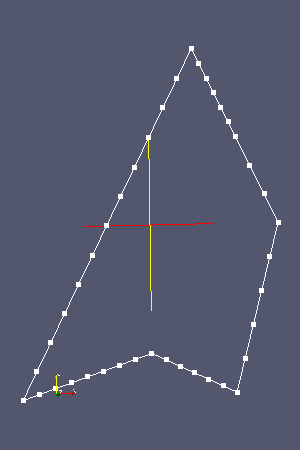
\includegraphics[scale=0.3]{snapshot2.png}
\end{frame}




\section{Ergebnisse}


\begin{frame}[fragile]
	\frametitle{Ende}
	Der Quellcode und diese Pr\"astentation sind zu finden auf
	\begin{verbatim}
		https://github.com/stev47/cp/tree/master/projekt2
	\end{verbatim}
\end{frame}




\end{document}
